\documentclass[12pt]{article}%
\usepackage{amsfonts}
\usepackage{fancyhdr}
\usepackage{comment}
\usepackage[a4paper, top=2.5cm, bottom=2.5cm, left=2.2cm, right=2.2cm]%
{geometry}
\usepackage{times}
\usepackage{amsmath}
\usepackage{changepage}
\usepackage{stfloats}
\usepackage{amssymb}
\usepackage{graphicx}
\usepackage{indentfirst}
\setlength{\parindent}{2em}
\setcounter{MaxMatrixCols}{30}
\newtheorem{theorem}{Theorem}
\newtheorem{acknowledgement}[theorem]{Acknowledgement}
\newtheorem{algorithm}[theorem]{Algorithm}
\newtheorem{axiom}{Axiom}
\newtheorem{case}[theorem]{Case}
\newtheorem{claim}[theorem]{Claim}
\newtheorem{conclusion}[theorem]{Conclusion}
\newtheorem{condition}[theorem]{Condition}
\newtheorem{conjecture}[theorem]{Conjecture}
\newtheorem{corollary}[theorem]{Corollary}
\newtheorem{criterion}[theorem]{Criterion}
\newtheorem{definition}[theorem]{Definition}
\newtheorem{example}[theorem]{Example}
\newtheorem{exercise}[theorem]{Exercise}
\newtheorem{lemma}[theorem]{Lemma}
\newtheorem{notation}[theorem]{Notation}
\newtheorem{problem}[theorem]{Problem}
\newtheorem{proposition}[theorem]{Proposition}
\newtheorem{remark}[theorem]{Remark}
\newtheorem{solution}[theorem]{Solution}
\newtheorem{summary}[theorem]{Summary}
\newenvironment{proof}[1][Proof]{\textbf{#1.} }{\ \rule{0.5em}{0.5em}}

\usepackage{mathtools}

\newcommand{\Q}{\mathbb{Q}}
\newcommand{\R}{\mathbb{R}}
\newcommand{\C}{\mathbb{C}}
\newcommand{\Z}{\mathbb{Z}}

\begin{document}

\title{MATH2040C Homework 6}
\author{ZHENG Weijia (William, 1155124322)}
\date{April 9, 2021}
\maketitle



\section{Section 6.1, Q8}

\begin{figure}[htp]
    \centering % 图片居中
    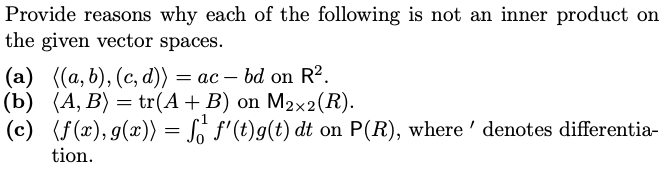
\includegraphics[width = 16cm]{img/Q1.png}
    \caption{Section 6.1 Q8}
    \label{fig:figure1label}
\end{figure}

\subsection{(a)}
Suppose this is an inner product. Then $\langle\, x,x \rangle \geq 0$ should hold $\forall x \in \mathbb{R}^2.$

Let $x=(1,10).$ Then $\langle\, x,x \rangle=\langle\, (1,10),(1,10) \rangle=1^2-10^2=-99<0.$

Therefore, this is not an inner product.

\subsection{(b)}
Suppose this is an inner product. Then $\langle\, x,x \rangle \geq 0$ should hold $\forall x \in M_{2\times 2}(R).$

Let $x=\begin{pmatrix} -1&0\\0&-1\end{pmatrix}$. Then $$\langle\, x,x \rangle=tr(x+x)=-2-2=-4<0.$$

Therefore, this is not an inner product.

\subsection{(c)}
Suppose this is an inner product. Then $\forall f,g \in P(\mathbb{R}), \overline{\langle\, g,f \rangle}=\langle\, f,g \rangle$ should hold.

Let $f(x)=x, g(x)=x^2+x.$

Then $$\langle\, f,g \rangle=\int_{0}^{1} 1(x^2+x) \,dx=\frac{5}{6}.$$

$$\overline{\langle\, g,f \rangle}=\overline{\int_{0}^{1} (2x+1)x \,dx}=\frac{7}{6}.$$

Therefore $\overline{\langle\, g,f \rangle} \neq \langle\, f,g \rangle$ for some $f,g \in P(\mathbb{R}).$

Hence, this is not an inner product.

Done.

\section{Section 6.1, Q17}
\begin{figure}[htp]
    %\centering % 图片居中
    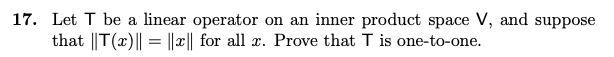
\includegraphics[width = 15cm]{img/Q2.png}
    \caption{Section 6.1 Q17}
    \label{fig:figure1label}
\end{figure}

Note that because we have $||T(x)||=||x||.$ Then $\forall x\in V$, with $x\neq 0$ we have $$||T(x)||=||x||>0.$$

Therefore $x\neq 0.$ 

Note that $||T(0)||=||0||=0$, which implies $$T(0)=0.$$

Hence $N(T)=\{0\}.$

Hence, $T$ is one-to-one.

Done.


\end{document}
